\documentclass[../Elmag-labhefte-2020.tex]{subfiles}

\begin{document}


\chapter{KRAFT PÅ STRØMFØRENDE LEDER\label{ch.kraft} }

\subsection*{Mål}

Du skal i denne laboratorieoppgaven
%
\begin{itemize}
 \item utvikle dine ferdigheter i å dokumentere laboratoriearbeid med labjournalen
    \item studere kraften mellom en strømførende leder og et konstant magnetfelt, 
    \item få erfaring med framstilling av resultater fra presisjonsmålinger, 
    \item utføre databehandling av måleresultatene vha. regresjonsanalyse i Python (minste kvadraters metode). % og/eller Excel
\end{itemize}
%


%**********************************************
\section{Teoretisk bakgrunn}
%**********************************************

%Teorien presenteres i samband med beregningsoppgavene nedenfor. Forøvrig vises til lærebok og forelesningene i elektromagnetisme.


%%%%%%%%%%%%%%%%%%%%%%%%%%%%%%%%%%%%%%%%%%%%%%%%%%%
%\section{Beregningsoppgaver \label{ch.kraft.beregn}}
%%%%%%%%%%%%%%%%%%%%%%%%%%%%%

\subsection{Kraft på en leder \label{ch.kraft.beregn1} }
%%%%%%%%%%%%%%%%%%%%%%%%%%%%%
Et elektron med ladning $q = -e$ som beveger seg med en hastighet $\va*{v}$ i en leder som er plassert i et magnetfelt $\va*{B}$ vil bli påvirket av en kraft ifølge Lorentzkraften 
\begin{equation}
    \va*{F} = q \va*{v} \cross \va*{B}.
\end{equation}
%
 Den totale kraften på en strømførende leder i et magnetfelt blir den resulterende kraften på alle elektronene i lederen:
\begin{equation}
    \va*{F} = q (\va*{v}_d \cross \va*{B} ) n A \ell,
\end{equation}
%
hvor $\ell$ er lengden av lederen, $A$ er tverrsnittsarealet, $n$ er elektrontettheten og følgelig blir $n A \ell$ lik totalt antall elektroner i lederen. Hastigheten $\va*{v}_d$ må forstås som gjennomsnittshastigheten (drifthastigheten) til elektronene. 
Den elektriske strømmen i en leder er definert som 
\begin{equation}
    I = nqv_d A ,
\end{equation}
og følgelig vil kraften kunne uttrykkes
\begin{equation}
    \va*{F} = I\va*{\ell} \cross \va*{B},
\end{equation}
%
hvor $\va*{\ell}$  må oppfattes som en vektor med retning langs lederen i strømretningen. Skrevet ut på skalar form blir likningen
\begin{equation}
    F = I\ell B \sin \theta,
    \label{eq:kraft.5}
\end{equation}
hvor $\theta$ er vinkelen mellom magnetfeltet og positiv strømretning i lederen. Når lederretningen er vinkelrett på magnetfeltretningen er $\theta = \pi/2$, og likning \eqref{eq:kraft.5} forenkles til 
\begin{equation}
    F = I\ell B.
    \label{eq:kraft.6}
\end{equation}
%
Kraften på en strømførende leder i et magnetfelt kan måles med oppstillingen i figur \ref{kraft.fig1}.
\begin{figure}[tbh]
    \centering
    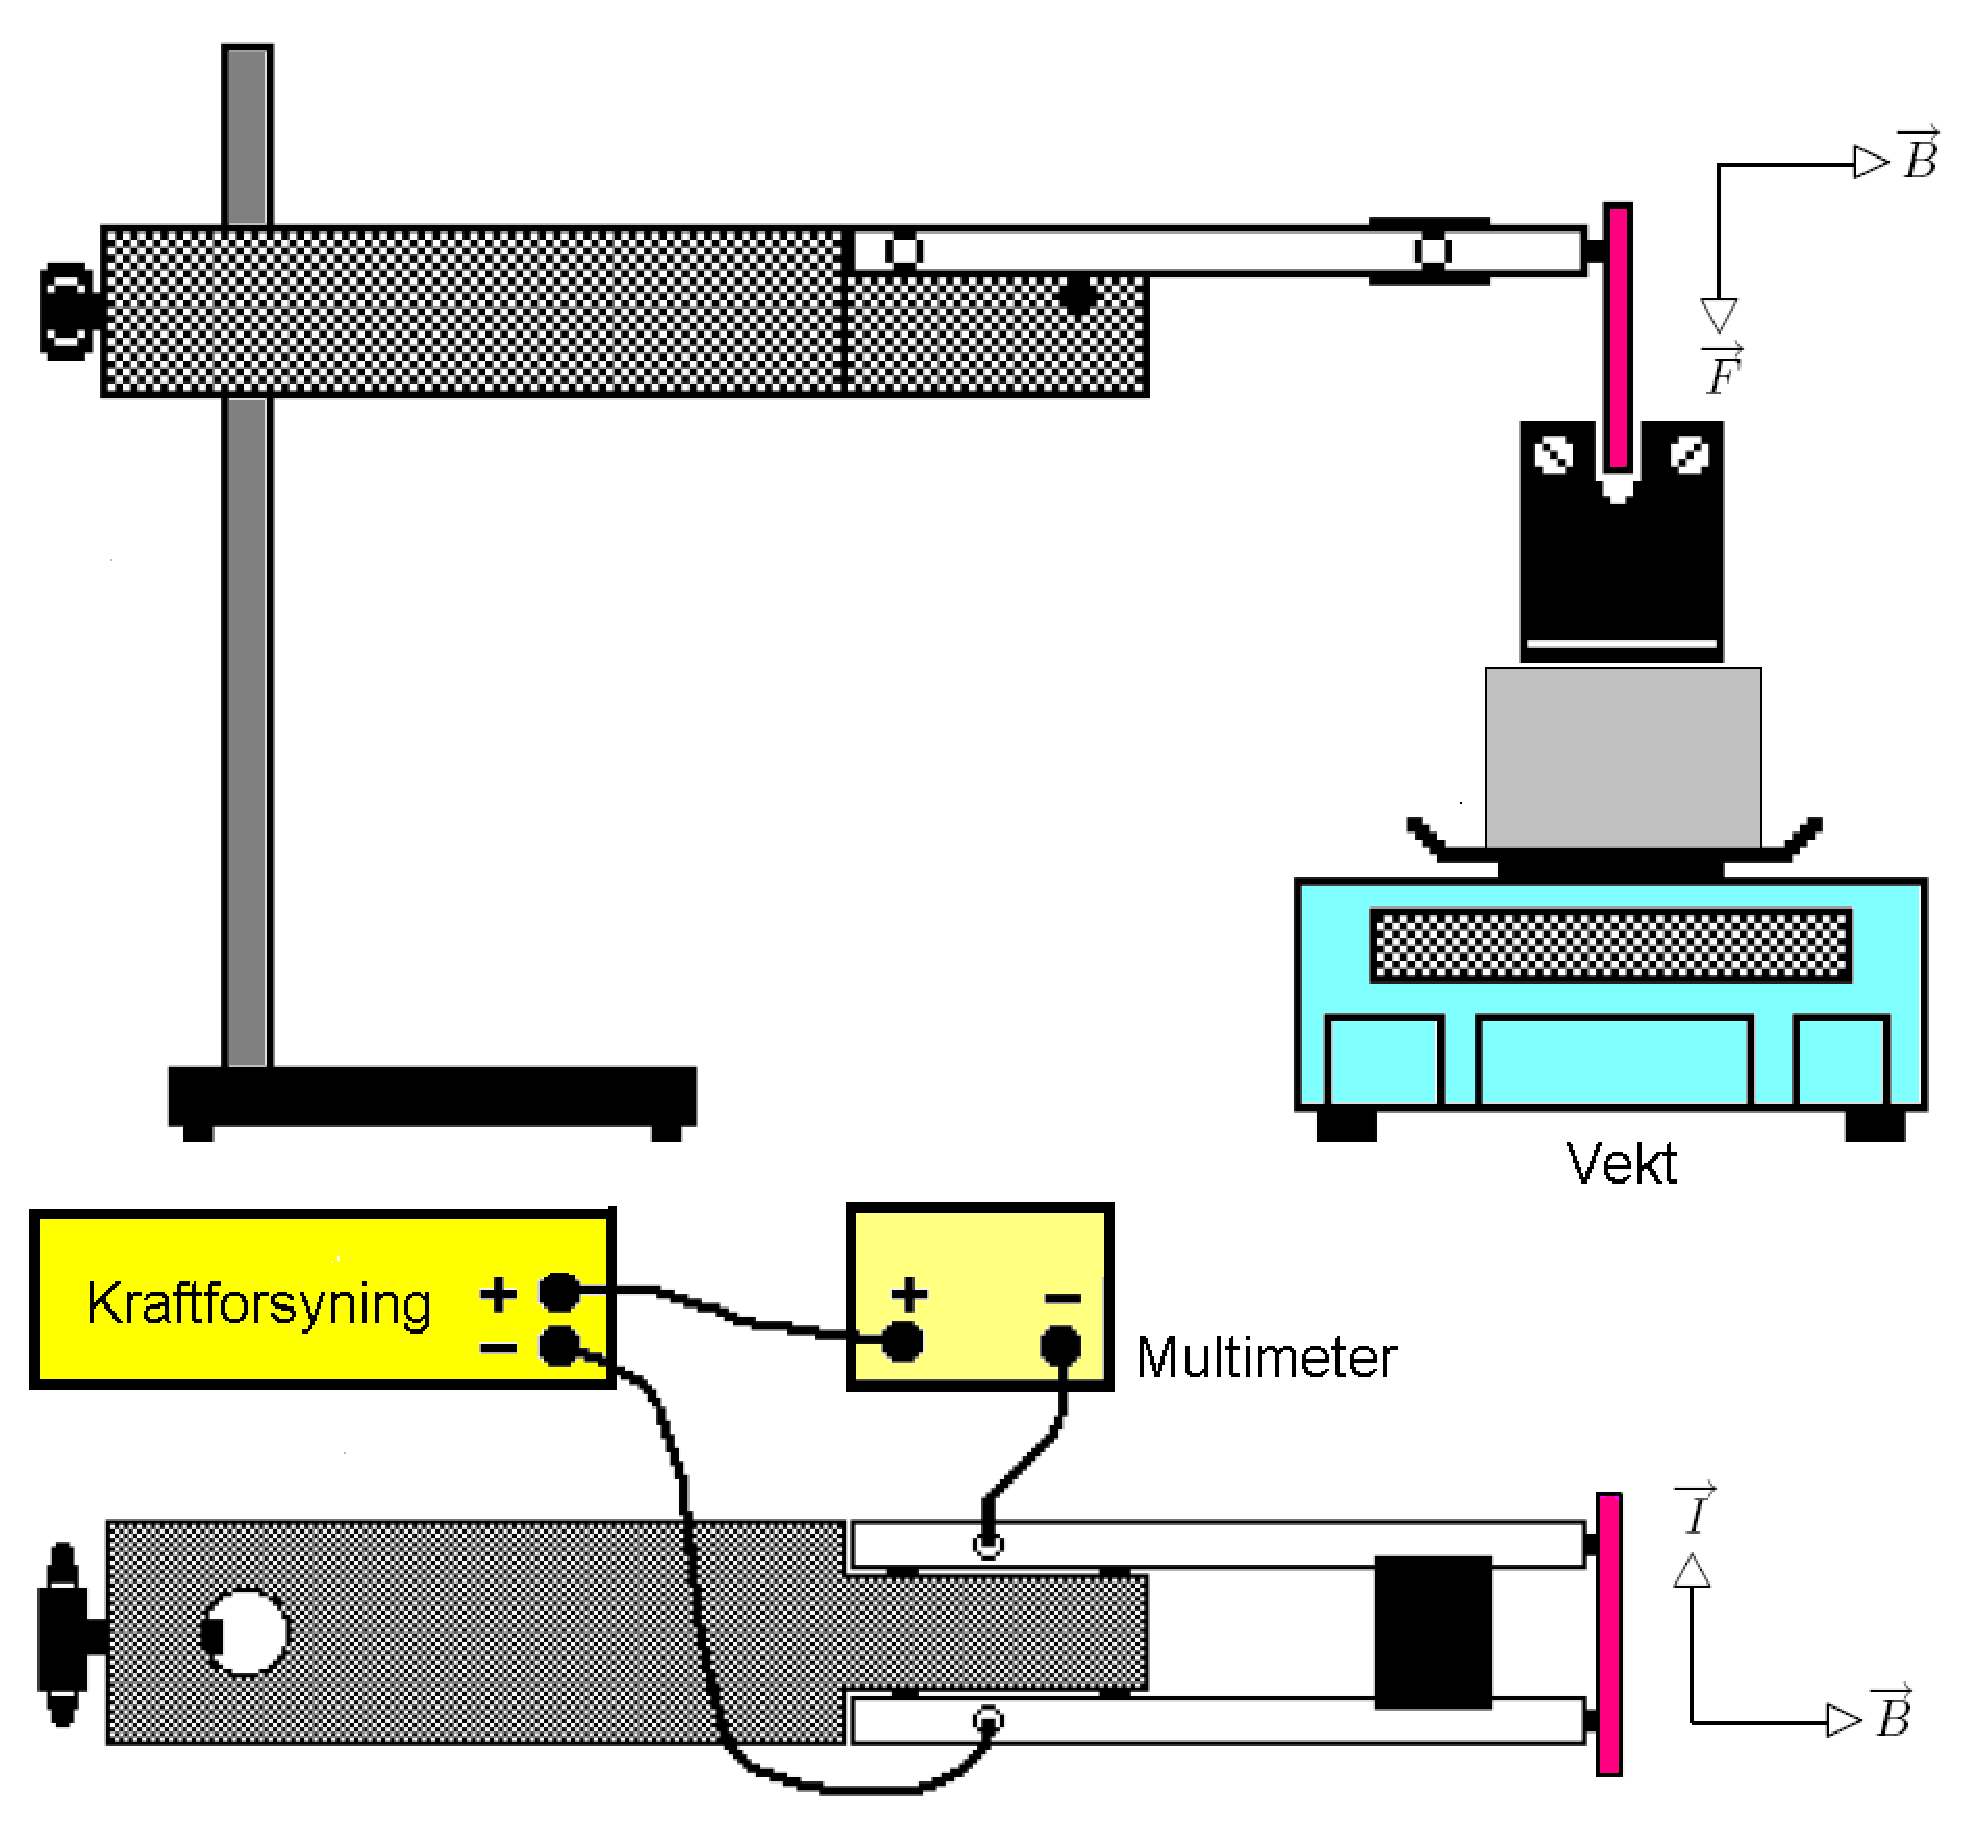
\includegraphics[width=10cm,height=9.28cm,keepaspectratio]{KraftFig1.eps}
    \caption{%
        Prinsippskisse for oppstilling for måling av kraft på en strømførende leder. Øverst vises oppsettet sett ifra siden, og nederst vises oppsettet sett ovenfra.
    }
    \label{kraft.fig1}
\end{figure}
Magneten hviler på vekta, mens den strømførende lederen er fastmontert uavhengig av vekta. Kraftvirkning mellom lederen og magneten vil bli registrert som utslag på vekta. Vekta er imidlertid kalibrert og gradert til å måle masse $M$ i gram idet en viss verdi for tyngdeakselerasjon $g$ er antatt. Sammenhengen mellom kraft og masse er som kjent gitt av 
\begin{equation}
    F = M g, 
    \label{eq:kraft.7}
\end{equation}
slik at fra likning \eqref{eq:kraft.5} vil vi få uttrykk for vektas utslag:
\begin{equation}
    M = \frac{I \ell B}{g} \sin \theta.
    \label{eq:kraft.8}
\end{equation}
%Når $\theta = \pi/2$, kan likning \eqref{eq:kraft.8} omskrives som
%\begin{equation}
%    M (I) = a_1^\prime I,
%    \quad \bigl 
%    (a_1^\prime = \ell B/g \bigr),
%    \label{eq:kraft.8a}
%\end{equation}
%eller som
%\begin{equation}
%    M(\ell) = b_1^\prime \ell,
%    \quad \bigl 
%    ( b_1^\prime = IB/g\bigr ).
%    \label{eq:kraft.8b}
%\end{equation}

%\subsection{Kraft sfa. strøm og lederlengde \label{ch.kraft.beregn2}}
%%%%%%%%%%%%%%%%%%%%%%%%%%%%%

%{\itsf 1. Bruk Excel eller MATLAB til å sette opp et kurvediagram over vekta $M$ i gram som funksjon av trådlengden $\ell$ langs $x$-aksen i området 0 til 100 mm når du antar $B$ = 700 gauss. Lag fem kurver i diagrammet der strømmen er parameter: $I = $ 1, 2, 3, 4 og 5 A.
%}

%Bruk likning (\ref{eq:kraft.8}) med $\sin \theta = 1$ og $g = 9,82 \times 10^{-3} $ N/g. 


%\textbf{2. Sett opp et annet kurvediagram med samme størrelse langs $y$-aksen men med strømmen $I$ i området 0 til 5 A langs $x$-aksen. Lag fire kurver med lengden av tråden som parameter: $\ell = $ 12,5; 22,5; 32,5 og 42 mm.} 

\subsection{Kraft sfa. vinkelen  \label{ch.kraft.beregn3}}
%%%%%%%%%%%%%%%%%%%%%%%%%%%%%

Du erstatter lederen med en spole som vist i figur \ref{kraft.fig2} hvor vinkelen mellom spoleaksen og magnetfeltretningen er variabel. Spolen har $N = 10$ rektangulære viklinger med sidelengder \SI{11}{\mm} og kun den nedre delen av spolen ligger i magnetfeltet slik at kraften bare virker på den nedre horisontale del av viklingene, dvs.\ total lengde \SI{110}{\mm}. Vinkelen mellom strømretningen og magnetfeltet er $\theta$ og inngår i likningen for beregning av kraften.

\begin{figure}[h]
    \setlength{\unitlength}{1mm}
    \begin{picture}(120,60)(-30,0)
        %\multiput(30,12.5)(6,6){3}{\line(1,1){5}} 
        
        \multiput(30.3,12.3)(0.75,0.75){26}{$\cdot$} %\multiput(30,12.5)(0.75,0.75){26}{\circle{0.5}}
        
        \linethickness{0.2mm}
        \newsavebox{\dumb}
        \savebox{\dumb}(10,10)[l]{
            \put(28,-20){\line(-3,2){18}} %\put(10,10){\line(1,-2){15}} 
            \put(27.4,-20.8){\tiny$\otimes$}%\put(28,-20){\circle}
            %\put(10,-8){\circle{1.59}} %\put(10,-8){\circle{1.59}} 
            %\put(9.5,-9){$\cdot$}
            %\put(27.1,-20.5){\small$\times$}
            \put(8.7,-8.2){\tiny$\odot$}
        } 
        \multiput(20,20)(1.2,1.2){10}{\usebox{\dumb}} 
        \qbezier(32,48)(28,43)(31,39)
        \put(30.5,36.5){$\searrow$}
        \thicklines
        \put(26,15){\line(0,1){30}} 
        \put(26,15){\line(-1,0){10}} 
        \put(26,45){\line(-1,0){10}} 
        
        
        \put(51,33.3){\vector(-3,2){9.6}}%11 mm arrow northwest
        \put(51,33.3){\vector(3,-2){9}}%11 mm arrow southeast
        \put(35,35.5){\vector(1,1){4.5}}
        \put(35,35.5){\vector(-1,-1){6.5}}
        %\color{black}
        \put(32,48){10 viklinger}
        
        
        \put(62,15){\line(0,1){30}} 
        \put(62,15){\line(1,0){10}} 
        \put(62,45){\line(1,0){10}} 
        
        \put(18,28){\huge N}
        \put(68,28){\huge S}
        
        \put(50,35){$\swarrow$}
        \put(48,41){$\underbrace{\;11 \mbox{mm}\;}$}
        
        \put(30,12.5){\vector(1,0){20}} %B-vector
        \put(30,12.5){\vector(3,-2){15}} %I-vector
        \qbezier(40,12.5)(41,10)(39,7) %Arc for theta
        %
        
        %\put(30,12.5){\line(1,1){20}} 
        
        \put(51,11){$\va*{B}$}
        \put(46,3){$\va*{I}$}
        \put(41,8){$\theta$}
    \end{picture}
    \caption{%
        Dreibar spole plassert i magnetbrønnen, sett ovenfra. Kun den nedre delen av spolen ligger i magnetfeltet og de vertikale lederne (markert med $\times$ og $\cdot$ på figuren) er påvirket av krefter i horisontal retning og som innbyrdes nuller hverandre ut.
    }
    \label{kraft.fig2}
\end{figure}

%\begin{figure}[h]
%\begin{center}
%\vspace{1cm}
%\hspace{-4cm}
%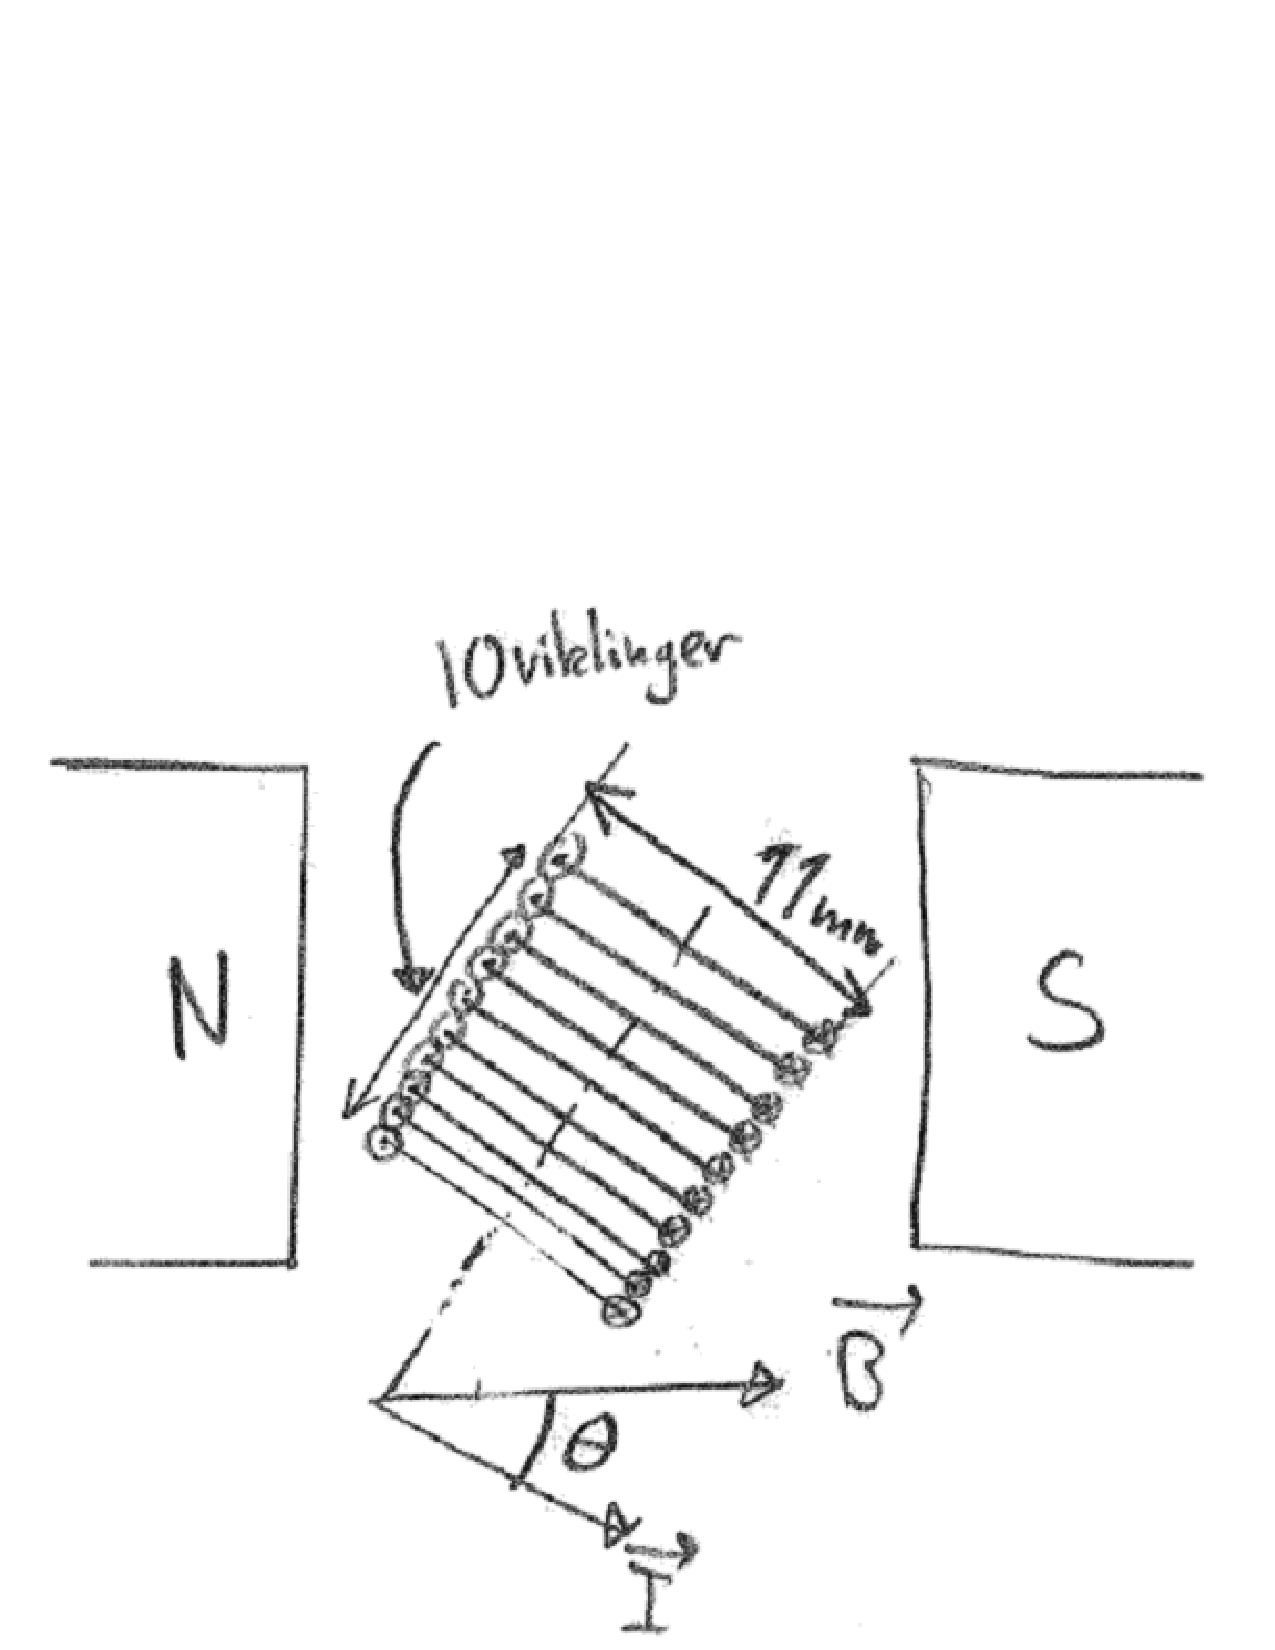
\includegraphics[bb=0 0 450 412,width=6cm,height=9cm,keepaspectratio]{KraftFig2}
%\vspace{-8mm}
%\end{center}
%\caption{\sf Dreibar spole plassert i magnetbrønnen, sett ovenfra. Kun den nedre delen av spolen ligger i magnetfeltet og de vertikale lederne (markert med $\times$ og $\cdot$ på figuren) er påvirket av krefter i horisontal retning og som innbyrdes nuller hverandre ut.}
%\label{kraft.fig2}
%\end{figure}


%{\itsf 2. Bruk Excel eller MATLAB til å sette opp et kurvediagram over vekta $M$ i gram som funksjon av vinkelen $\theta$ i grader i området -90$^\circ$ til +90$^\circ$. Lag to kurver i diagrammet med strømmen som parameter: $I = $ 2 og 4 A. Bruk trådlengde 11 mm $\times$ 10 = 110 mm og  $B$ = 200 gauss.
%}

%\subsection{Elektrisk motor  \label{ch.kraft.beregn4}}
%%%%%%%%%%%%%%%%%%%%%%%%%%%%%

%}


\section{Forhåndsoppgaver}
Gjør deg kjent med scriptet for lineær kurvetilpasning som ligger på Blackboard (Jupyter notebook). Det blir utdelt to eksempler på datasett som kan brukes til å teste. 

%%%%%%%%%%%%%%%%%%%%%%%%%%%%%%%%%%%%%%%%%%%%%%%%%%%%%%%%%%%%%%%%%%%%%%%%%%%%%%
\section{Eksperimentelt \label{ch.kraft.eksp} }
%%%%%%%%%%%%%%%%%%%%%%%%%%%%%%%%%%%%%%%%%%%%%%%%%%%%%%%%%%%%%%%%%%%%%%%%%%%%%%

%%%%%%%%%%%%%%%%%%%%%%%%%%%%%%%%%%%%%%%%%%%%%%%%%%%%%%%%%%%%%%%%%%%%%%%%%%%%%%
\subsection{Apparatur}
%%%%%%%%%%%%%%%%%%%%%%%%%%%%%%%%%%%%%%%%%%%%%%%%%%%%%%%%%%%%%%%%%%%%%%%%%%%%%%

Følgende instrumenter inngår i oppstillingen:
\vspace{-4mm} 
\begin{itemize}
    \item \textbf{Elektromagnetisk vekt.} Mettler Mod. PM480.  Område: 0-\SI{400}{\g}. Presisjon: $\pm \SI{1}{\milli\g}$, eller Mettler Mod. PB-SDR/FACT. Område 0-\SI{60}{\g} $\pm$ \SI{1}{\milli\g}/70-\SI{310}{\g} $\pm$ \SI{8}{\milli\g}.
    \item \textbf{Stativ for strømbaner.} Pasco SF-8607. 
    \item \textbf{Faste strømbaner} og \textbf{magnetbrønn} med variabelt magnetfelt fra \SI{125}{\G} til \SI{750}{\G} i trinn på \SI{125}{\G}.  Fabrikat og type: Pasco SF-8607. Max 5A
    \item \textbf{Roterbar spole} med 10 rektangulære viklinger horisontal, dimensjon 11 $\times$ \SI{23}{\mm},  med tilhørende magnetbrønn med magnetfelt lik ca \SI{250}{\G}.  Max 5A.
    Fabrikat og type: Pasco SF-8608.
    \item \textbf{Kraftforsyning.} Fredriksen Mod. 364000. Område: 0-\SI{24}{\volt} 0-\SI{10}{\ampere}. Brukes som strømkilde.
    \item \textbf{Multimeter.} Keithley 175A eller GW instek GDM-8246.
    \item \textbf{Gaussmeter.} Magnetic Instruments RFL, Mod. 912. \\
    Måleområde: \(\SI{0.01}{\G}-\SI{100}{\kilo\G}\). \\
    Presisjon: \(\pm\) (0.4 \% av avlesning + 0.1 \% av område + 1 i siste siffer). \\
    Transversal probe.
    \item \textbf{Skyvelære.}
\end{itemize}

Vekta er et presisjonsinstrument som du må behandle med forsiktighet. Pass spesielt på å unngå støt mot veiepannen under montering og demontering av oppstillingen.  Vekta bygger på en elektromagnetisk veiemetode etter kompensasjonsprinsippet slik at veiepannen ikke forandrer stilling under veiingen. Dette er viktig for målingene våre.

%Figuren til venstre viser vektas oppbygging skjematisk: En spole er viklet på veiepannen. Spolen er senket ned i en sirkulær permanent magnetbrønn som gir et konstant magnetfelt.  Når veiepanna blir belastet genereres det en strøm i spolen som i vekselvirkning med magnetfeltet gir en kraft som kompenserer for bevegelsen av veiepannen. Veiepannens posisjon blir overvåket av en optisk sensor som er koplet i en servosløyfe som regulerer strømmen i spolen slik at posisjonen ikke forandres.

Lederne som brukes i eksperimentene er bygget opp som moderne elektroniske kretskort med smale strømbaner av kobber som er dampet på glassfiberarmerte polyesterplater. For å forhindre oksidering av kobberoverflata er den dekket med tinn. Totalt inneholder instrumentoppstillingen seks faste strømbaner av forskjellig lengde, hvor fire er enkle og to er doble.

Som magnetfeltkilde brukes en magnetbrønn bygget opp av seks like permanentmagneter. Feltet i brønnen kan varieres ved å fjerne magnetene en etter en. 

For å undersøke kraften sfa. vinkelen mellom feltretning og strømretning brukes i siste eksperiment en roterbar spole med egen magnetbrønn. 



\subsection{Kraft sfa. strømmen}
%%%%%%%%%%%%%%%%%%%%%%%%%%%%%%%%%%%%%

Oppgave: \\
{\itsf Undersøk hvordan kraften mellom en tynn strømførende leder og et magnetfelt med retning vinkelrett på lederen avhenger av strømmen i lederen.}

Forslag til framgangsmåte:
%
\vspace{-4mm} 
\begin{itemize}
    \item Velg en av strømbanene og mål lengden $\ell$ og bredden $t$ av strømbanen med skyvelære. (Pass på at du ikke skader strømbanen med skyvelæret.) Definer foreløpig strøm\-banens lengde som ytre dimensjon i lengderetningen.  %figur?
    Seinere får du anledning til å revurdere denne definisjonen. 
     
    \item Klargjør kraftforsyningen: Sjekk at den er slått av og strøm og spenning er sett til 0. 
    \item bruk multimeteret for måling av strømen
    \item Kople opp strømkretsen som vist i figur \ref{kraft.fig1}. .
    \item Sjekk nivelleringen av vekta (libelle bak, juster føtter) og slå deretter vekta på.
    \item Still magnetbrønnen midt på vekta med den perforerte sylinderen mellom magnetbrønnen og vekta. % som vist i figur.
    (Den perforerte sylinderen er satt inn for å øke avstanden mellom magnetbrønnen og vekta for å unngå at magnetfeltet fra magnetbrønnen forstyrrer vekta.) 
    \item Juster posisjonen til lederen i forhold til magnetbrønnen slik at den ligger midt i magnetfeltet.
    %\item Be læreren om å godkjenne oppstillingen.
    \item Nullstill vekta.
    MERK: For å være helt sikker på at det ikke går strøm i kretsen under nullstillingen bør du bryte strømkretsen ved å trekke ut en av kontaktene mens du nullstiller. 
    \end{itemize}
    
Målingen can nå startes. Kraftforsyningen skal være strømstyrt, men kraftforsyningen kan levere opp til \SI{10}{\ampere} mens \emph{strømbanen tåler maksimalt \SI{5}{\ampere}}. Det er ditt ansvar å passe på at strømbanen ikke blir overbelastet! Følg med på strømmåleren!

målingen skal gir svar på det følgende:
\begin{itemize}
        \item Hva er sammenheng mellom vekta $M  = F/g$ sfa. strømmen $I$ i området 0-\SI{5}{\ampere}? Dokumenter måleresultatene i labjournalen og i en datafil. 
        %Ta ca 30 målepunkter fordelt over området men tettest med målinger ved lavere $I$-verdier. \\
        \item Hva skjer når du bytter polaritet på strømbanen? Får du et forventet resultat? 
    \item Hva skjer når du snur magneten?  Får du et forventet resultat? 
    \item Vis i en skisse strømretninger og kraftretninger og identifiser magnetpolene.
    %\item Juster oppstillingen din om nødvendig 
    %\item Foreta en ny nullstilling av vekta
    %\item Slå datamaskinen på og start Excel
     % eller regnearket
    %\item Lag graf for målt verdi og sammenlikn målt verdi med den teoretisk beregnede.
    \item Mål tilslutt magnetfeltet $B$ i magnetbrønnen med gaussmeteret.
\end{itemize}

\subsubsection{Analyse/diskusjon:}

\vspace{-4mm} 
\begin{itemize}
    \item Tilpass måledata til $M^\ast = a_0 + a_1 I$. Finn "beste" rette linje gjennom målepunktene vha. lineær regresjon og bestem stigningstallet $a_1$ og usikkerheten $\Delta a_1$.
    \item Beregn forventet stigningstall $a_1^\prime$ for $M(I)$ ved å bruke målte verdier for $\ell$ og $B$ og likning \eqref{eq:kraft.8}. Finn også usikkerheten $\Delta a_1^\prime$.
     %Bruk $g = 9,81 \cdot 10^{-3} $ N/g.  
    \item Er verdien av $a_1^\prime$ lik stigningstallet $a_1$ fra den eksperimentelle kurven innenfor usikkerheten? Hvis ikke, kan du forklare avviket?
    \item Plot avviket mellom målte verdier og verdier fra lineær regresjon for kraften som funksjon av strøm. Ser det ut som det er en lineær sammenheng mellom kraften og strømstyrken? (Tips: Se på hvordan målepunktene er fordelt rundt regresjonslinjen.) Dersom du antar at det er en lineær sammenheng, samsvarer størrelsen på avvikene med målenøyaktigheten til vekten?%Er verdien av $\Delta a_1$ i samsvar med instrumentenes målenøyaktighet? Vektas nøy\-aktighet er gitt i apparaturbeskrivelsen. Strømmen måles med en nøyaktighet på $\pm 1$~mA.
    \item Kan du, når du tar hensyn til resultatene fra feilanalysen, påstå at du har verifisert likning \eqref{eq:kraft.8}?
    \item Skriv ut kurvediagram og grafer og lim inn i journalen sammen med kommentarer.
\end{itemize}

\subsection{Kraft sfa. lengden \label{ch.kraft.lengde} }
%%%%%%%%%%%%%%%%%%%%%%%%%%%%%%%%%%%%%

Oppgave: \\
{\itsf Undersøk hvordan kraften på en tynn leder i et magnetfelt med retning vinkelrett på lederen avhenger av lengden av lederen.}

%Du kan eventuelt følge denne detaljerte framgangsmåten:
%
\begin{itemize}
\vspace{-4mm} 
    \item Oppsett og måling av kraften skjer som i oppgave ovenfør. 
    \\ VIKTIG: Reduser strømmen i kretsen til null hver gang du skifter leder. 
    %\item Mål vekta $M$ for hver av strømbanene ved fast strøm (f.eks.\ 2 A, maks.: 5 A) sfa. lengden $\ell$ på strømbanen 
    \item Mål lengden og bredden av hver strømbane så nøyaktig som mulig. Bruk ytre dimensjon for lengden. Legg merke til at to av strømbanene er doble. 
    % MERK: Strømbane SF 38, 39, 37 og 40 er enkle. Strømbane SF 41 og 42 er doble. Ta hensyn til dette når du bestemmer lengden av banene. 
    \item Dokumenter resultatene i labjournalen og i en datafil etterhvert som du måler.
\end{itemize}

\subsubsection{Analyse/diskusjon:}

\vspace{-4mm} 
\begin{itemize}
    \item Tilpass måledata til $M^\ast = b_0 + b_1\ell$. Finn "beste" rette linje gjennom målepunktene vha. lineær regresjon og bestem stigningstallet $b_1$ og usikkerheten $\Delta b_1$.
    \item Beregn forventet stigningstall $b_1^\prime$ for $M(\ell)$ ved å bruke målte verdier for $I$ og $B$ og likning \eqref{eq:kraft.8}. Finn også usikkerheten $\Delta b_1'$.
     %Bruk $g = 9,81 \cdot 10^{-3} $ N/g.  
    \item Ligger verdien av $b_1^\prime$ innenfor usikkerheten $b_1 \pm \Delta b_1$ fra den eksperimentelle kurve? Hvis ikke, kan du forklare avviket?
    %TIPS: Ladningene søker alltid å plassere seg lengst mulig fra hverandre (Coulombs lov). 
    %\item Forsøk en ny regresjon der du ikke legger regresjonslinja gjennom origo men med skjæringspunktet $b$ på $y$-aksen som variabel.%\footnote{Oppnås ved å velge logisk verdi ``1'' i tredje parameter til funksjonen RETTLINJE.}
    \item Ut fra dine resultater her, eventuelt revider definisjonen din av lederens lengde.
    \item Kan du, når du tar hensyn til resultatene fra feilanalysen, påstå at du har verifisert likning \eqref{eq:kraft.8}?
    \item Skriv ut kurvediagram og grafer og lim inn i journalen sammen med kommentarer.
\end{itemize}

%Dersom du nå har tid kan du undersøke avhengigheten av magnetfeltet $B$ ved å fjerne delmagneter fra magnetbrønnen.

\subsection{Kraft sfa. vinkelen}
%%%%%%%%%%%%%%%%%%%%%%%%%%%%%%%%%%%%%

Oppgave: \\
{\itsf Undersøk hvordan kraften på en tynn strømførende leder avhenger av vinkelen mellom lederen og magnetfeltet.}

Framgangsmåte:
%
\vspace{-4mm} 
\begin{itemize}
    \item Plasser den dreibare spolen på stativet og bruk den tilhørende magnetbrønnen.
    \item Mål vekta $M$ sfa. vinkelen $\theta$ mellom spolen og magnetfeltet ved fast strøm (f.eks. \SI{2}{\ampere}). 
    \item Dokumenter resultatene i labjournalen og i en datafil etterhvert som du måler. %Bruk regnearket du laget for teoretisk beregning av kraft sfa. vinkel i kap.\ \ref{ch.kurve.excel}.
    \item Lag en regresjonskurve på formen \(M^{*} = c_0 + c_1 \sin \theta\) for resultatene dine. Legg merke til av vi kan bruke lineær-regresjon for å tilpasse en sinus dersom vi bruker \(\sin \theta\) som \(x\)-verdier. 
    %(Bruke Python-skriptet fra kapittel \ref{ch.kurve.matlab}.)% eller en tilpasset versjon av Excel-regnearket fra kapittel \ref{ch.kurve.excel}.) %Sammenlign resultatene med de teoretiske verdier plottet inn i regnearket.
    \item Gjennomfør samme analyse / diskusjon som for tidligere målinger. 
\end{itemize}

\subsection{Generell diskusjon}
%%%%%%%%%%%%%%%%%%%%%%%%%%%%%%%%%%%%%

\vspace{-4mm} 
\begin{itemize}
%\item Sammenlign måleresultatene 
    \item Diskuter målenøyaktigheten i eksperimentet og dens innflytelse på mulighetene for sammenlikning med teorien. 
    \item Diskuter den mest riktige måten å angi lengden av lederen i oppgave \ref{ch.kraft.lengde}. Har du mulighet til å beregne en effektiv lengde ut fra eksperimentelle data?
    %\item Diskuter problemstillinger knyttet til problematikken verifisering / falsifisering av teorier. 
\end{itemize}


%%%%%%%%%%%%%%%%%%%%%%%%%%%%%%%%%%%%%%%%%%%%%%%%%%
\subsection{Avslutning}
%%%%%%%%%%%%%%%%%%%%%%%%%%%%%%%%%%%%%%%%%%%%%%%%%%

\begin{itemize}
    \item Slå av alle apparater, trekk ut alle ledninger og forlat plassen i minst like god orden som du fant den.
%\item Lever journalen til laboratorielæreren for godkjenning.
\end{itemize}

%%%%%%%%%%%%%%%%%%%%%%%%%%%%%%%%%%%%%%%%%%%%%%%%%%
%\section{Rapport}
%%%%%%
%I løpet av labbkurset for TFY4155/FY1003 Elektromagnetisme skal det skrives en individuell rapport, og den skal skrives for dette siste eksperimentet om kraft på en strømførende leder. Kravene til utforming og innhold for denne rapporten er i all hovedsak identiske som for rapporten du skrev i labbkurset for TFY4145/FY1001 Mekanisk fysikk. Før du setter i gang anbefaler vi derfor at du repeterer kapitlene i labbheftet for Mekanisk fysikk som omhandler rapportskriving, i tillegg til at du går gjennom tilbakemeldingene du fikk fra labbveileder for din forrige rapport. Labbveilederen i TFY4155/FY1003 Elektromagnetisme vil ha informasjon om detaljene rundt rapporten som skal skrives.

%Det følgende er en liste over de viktigste punktene rapporten må inneholde. Merk at listen ikke er uttømmende, og at listen heller ikke nødvendigvis spesifiserer hverken kapittelinndelingen eller rekkefølgen innad i kapitlene.
%\begin{description}
%  \item[Sammendrag] Skriv et par setninger om hva du har undersøkt, hvordan du har undersøkt det, og hva du fant ut. (Vær konkret når du oppgir de viktigste resultatene.)
%  \item[Innledning] Forsøk veldig kort å sette eksperimentet i sammenheng.
%  \item[Teori] Presenter kort den teorien og de likningene som er nødvendige for å forstå resultatene og diskusjonen.
%  \item[Metode/Apparatur] a) Figur med apparaturoppsettet. b) Beskrivelse av de viktigste punktene i gjennomføringen.
%  \item[Resultat] a) Presenter diagrammer med både målepunkter og den tilhørende kurvetilpasningen, både for kraft som funksjon av strøm, som funksjon av lengde, og som funksjon av vinkel. b) Sammenlign de teoretiske stigningstallene med dem du har funnet fra kurvetilpasningen, både for kraft som funksjon av strøm og som funksjon av lengde. Husk å ta hensyn til usikkerheter for alle størrelser. c) Presenter figurer som illustrerer avviket mellom kurvetilpasningen og målepunktene for kraft som funksjon av strøm og som funksjon av lengde.
%  \item[Diskusjon] a) Hvor sikkert kan du si at det er en lineær sammenheng mellom kraft og strøm og mellom kraft og lengde? Er konstantleddet fra kurvetilpasningen lik null? b) Hvilken definisjon bør du bruke for lengden på lederne? Kan du si noe om hva den effektive lengden er ut fra krysningspunktet mellom regresjonslinjen og x-aksen for kraft som funksjon av lengde? c) Er det noen ledere der målingene for kraft skiller seg ut fra trenden fra de øvrige lederne, hva kan årsaken til dette være, og hvordan kan en best håndtere dette avviket i analysen? d) Hvilke tilfeldige og systematiske feilkilder regner du som vesentlige i dette eksperimentet? 
%  \item[Konklusjon] Det viktigste spørsmålet du forsøker å besvare i dette eksperimentet er om du kan verifisere formelen for kraft på en strømførende leder, og det er dette konklusjonen bør gi et svar på. Husk på at konklusjonen skal komme som en logisk følge av diskusjonen og den foregående presentasjonen av resultatene.
%\end{description}

\end{document}